\begin{block}{Répartition des macro-structures}
	Programme temporel : \textbf{scénario}. 
	Annotations de groupes sur les éléments de cette structure : 
    
    \begin{figure}
        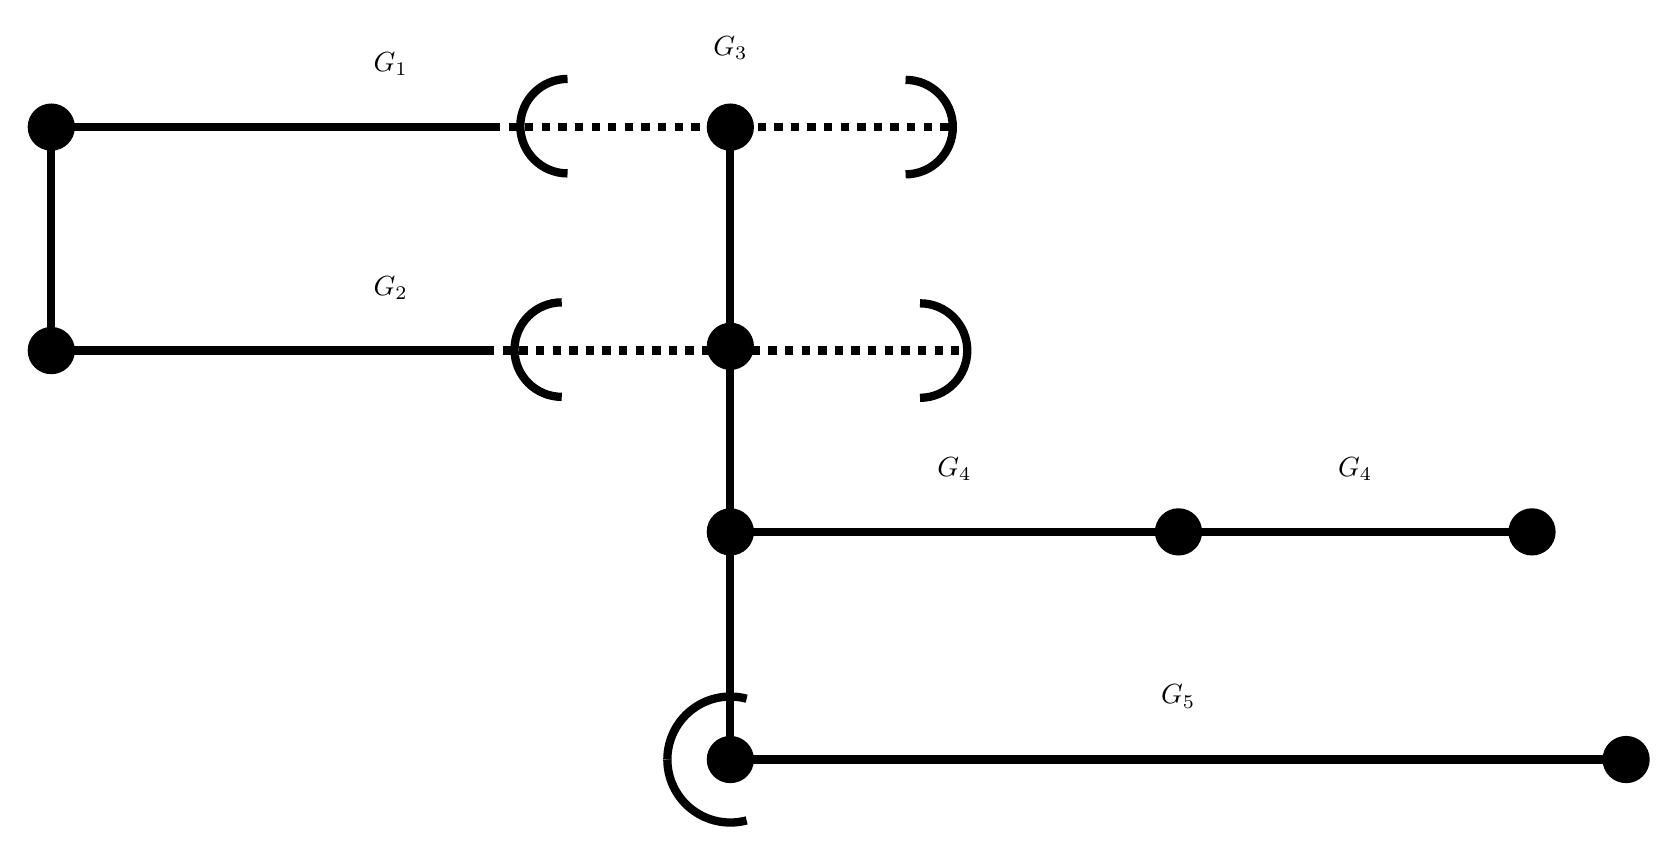
\begin{tikzpicture}[scale=4]
        \fill (0, 18.7148) circle (0.075) ; % State.0 
\fill (2.15596, 18.7148) circle (0.075) ; % State.1 
\fill (2.15596, 17.4296) circle (0.075) ; % State.2 
\fill (3.57887, 17.4296) circle (0.075) ; % State.3 
\fill (0, 18.0053) circle (0.075) ; % State.4 
\fill (2.15596, 18.0187) circle (0.075) ; % State.5 
\fill (2.15596, 16.7068) circle (0.075) ; % State.6 
\fill (5, 16.7068) circle (0.075) ; % State.7 
\fill (4.70124, 17.4296) circle (0.075) ; % State.8 
\draw[line width=3pt] (0, 18.7148)  -- (0, 18.0053) ; % TimeNode.0 
\draw[line width=3pt] (2.15596, 18.7148)  -- (2.15596, 16.7068) ; % numb47vine94 
\draw (2.15596, 18.9648) node {$G_3$}; % numb47vine94 
\draw[line width=3pt] (3.57887, 17.4296)  -- (3.57887, 17.4296) ; % faze44greg1 
\draw[line width=3pt] (5, 16.7068)  -- (5, 16.7068) ; % burp79lawn67 
\draw[line width=3pt] (4.70124, 17.4296)  -- (4.70124, 17.4296) ; % ness92piss60 
\draw[line width=3pt] (0, 18.7148)  -- (1.39908, 18.7148) ; % dido10rend91 
\draw[dashed,line width=3pt] (1.39908, 18.7148)  -- (2.86239, 18.7148) ; % dido10rend91 
\draw[line width=3pt] (1.63908, 18.8678) arc(90:270:0.15) ; % dido10rend91 
\draw[line width=3pt] (2.71239, 18.5648) arc(-90:90:0.15) ; % dido10rend91 
\draw (1.07798, 18.9148) node {$G_1$}; % dido10rend91 
\draw[line width=3pt] (2.15596, 17.4296)  -- (3.57887, 17.4296) ; % taut8hews94 
\draw (2.86742, 17.6296) node {$G_4$}; % taut8hews94 
\draw[line width=3pt] (0, 18.0053)  -- (1.38073, 18.0053) ; % ramp48lust85 
\draw[dashed,line width=3pt] (1.38073, 18.0053)  -- (2.90826, 18.0053) ; % ramp48lust85 
\draw[line width=3pt] (1.62073, 18.1583) arc(90:270:0.15) ; % ramp48lust85 
\draw[line width=3pt] (2.75826, 17.8553) arc(-90:90:0.15) ; % ramp48lust85 
\draw (1.07798, 18.2053) node {$G_2$}; % ramp48lust85 
\draw[line width=3pt] (2.15596, 16.7068)  -- (5, 16.7068) ; % dirt50gage22 
\draw (3.57798, 16.9068) node {$G_5$}; % dirt50gage22 
\draw[line width=3pt] (3.57887, 17.4296)  -- (4.70124, 17.4296) ; % viva88lint42 
\draw (4.14006, 17.6296) node {$G_4$}; % viva88lint42 
\draw[line width=3pt] (1.95596, 16.7068)  -- (1.95596, 16.7068) ; % sill78hues28 
\draw[line width=3pt] (1.95596, 16.7068) arc(180:75:0.2) ; % sill78hues28 
\draw[line width=3pt] (1.95596, 16.7068) arc(180:285:0.2) ; % sill78hues28 

        \end{tikzpicture}
        \caption{Les annotations $G_{1..5}$ s'appliquent récursivement sur les contenus}
    \end{figure}
	Trois modes d'exécution : 
	\begin{itemize}
		\item \textbf{Exécution indépendante}~:chaque client du groupe exécute le scénario à son rythme.
		\item \textbf{Partage complet}~: toutes les machines partagent la même ligne temporelle.
		\item \textbf{Partage mixte}~: certaines branches peuvent être exécutées par certains clients.
	\end{itemize}
    
    \begin{figure} \hspace*{-11cm}
        \begin{tabular}{L{3.5em}R{0.3\textwidth}}
            Racine: & 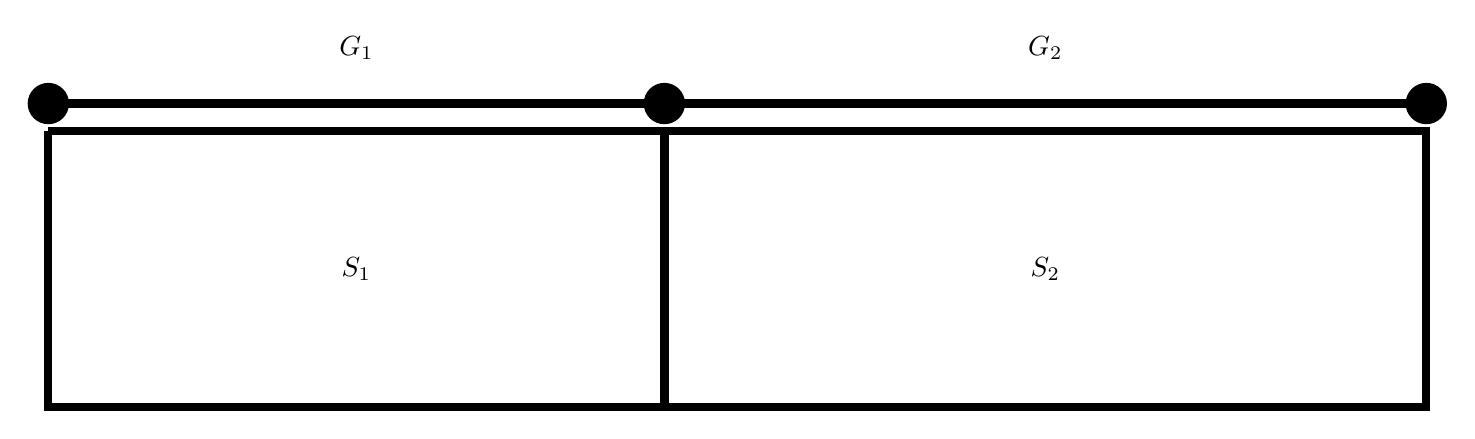
\begin{tikzpicture}[scale=3.5]
            \fill (0, 2.20767) circle (0.075) ; % State.1 
\fill (2.23529, 2.20767) circle (0.075) ; % State.2 
\fill (5, 2.20767) circle (0.075) ; % State.3 
\draw[line width=3pt] (0, 2.23364)  -- (0, 2.20767) ; % TimeNode.0 
\draw[line width=3pt] (2.23529, 2.20767)  -- (2.23529, 2.20767) ; % nook18bout42 
\draw[line width=3pt] (5, 2.20767)  -- (5, 2.20767) ; % nato89loop85 
\draw[line width=3pt] (0, 2.20767)  -- (2.23529, 2.20767) ; % step8duct27 
\draw (1.11765, 2.40767) node {$G_1$}; % step8duct27 
\draw[line width=3pt] (0, 2.10767)  -- (2.23529, 2.10767)  -- (2.23529, 1.10767)  -- (0, 1.10767)  -- (0, 2.10767) ;
\draw (1.11765, 1.60767) node {$S_1$}; % S_1 
\draw[line width=3pt] (2.23529, 2.20767)  -- (5, 2.20767) ; % what68step1 
\draw (3.61765, 2.40767) node {$G_2$}; % what68step1 
\draw[line width=3pt] (2.23529, 2.10767)  -- (5, 2.10767)  -- (5, 1.10767)  -- (2.23529, 1.10767)  -- (2.23529, 2.10767) ;
\draw (3.61765, 1.60767) node {$S_2$}; % S_2 

            \end{tikzpicture} \\
            $S_1$: & 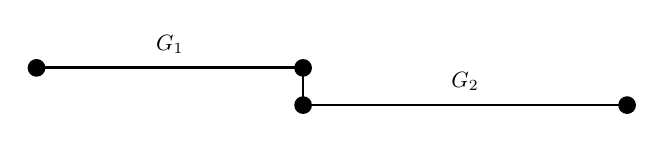
\begin{tikzpicture}[scale=1.5, every node/.style={scale=0.8}]
            
\fill (0, 9.28641) circle (0.075) ; % State.1 
\fill (2.25694, 9.28641) circle (0.075) ; % State.2 
\fill (2.25694, 8.97129) circle (0.075) ; % State.3 
\fill (5, 8.97129) circle (0.075) ; % State.4 
\draw[line width=1pt] (2.25694, 9.28641)  -- (2.25694, 8.97129) ; % loge35long20 
\draw[line width=1pt] (5, 8.97129)  -- (5, 8.97129) ; % wire36tick25 
\draw[line width=1pt] (0, 9.28641)  -- (2.25694, 9.28641) ; % sack65taft69 
\draw (1.12847, 9.48641) node {$G_1$}; % sack65taft69 
\draw[line width=1pt] (2.25694, 8.97129)  -- (5, 8.97129) ; % loon80rink81 
\draw (3.62847, 9.17129) node {$G_2$}; % loon80rink81 

            \end{tikzpicture} \\
            $S_2$: & 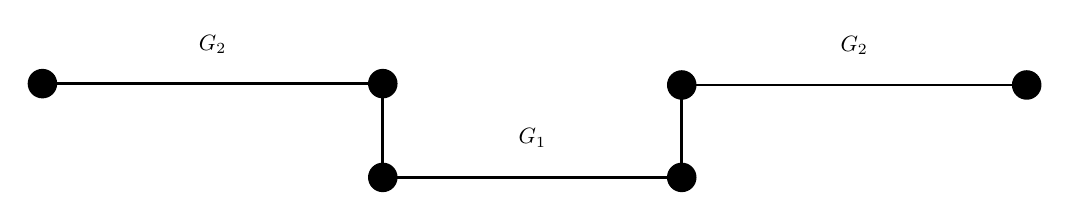
\begin{tikzpicture}[scale=2.5, every node/.style={scale=0.8}]
            \fill (0, 9.56564) circle (0.075) ; % State.0 
\fill (1.72897, 9.56564) circle (0.075) ; % State.1 
\fill (1.72897, 9.08927) circle (0.075) ; % State.2 
\fill (3.24766, 9.08927) circle (0.075) ; % State.3 
\fill (3.24766, 9.55873) circle (0.075) ; % State.4 
\fill (5, 9.55873) circle (0.075) ; % State.5 
\draw[line width=1pt] (0, 9.56564)  -- (0, 9.56564) ; % TimeNode.0 
\draw[line width=1pt] (1.72897, 9.56564)  -- (1.72897, 9.08927) ; % jogs95rang7 
\draw[line width=1pt] (3.24766, 9.55873)  -- (3.24766, 9.08927) ; % haul29dade96 
\draw[line width=1pt] (5, 9.55873)  -- (5, 9.55873) ; % vane42mets16 
\draw[line width=1pt] (0, 9.56564)  -- (1.72897, 9.56564) ; % scum85toss49 
\draw (0.864486, 9.76564) node {$G_2$}; % scum85toss49 
\draw[line width=1pt] (1.72897, 9.08927)  -- (3.24766, 9.08927) ; % woof52dyad40 
\draw (2.48832, 9.28927) node {$G_1$}; % woof52dyad40 
\draw[line width=1pt] (3.24766, 9.55873)  -- (5, 9.55873) ; % eben10crux7 
\draw (4.12383, 9.75873) node {$G_2$}; % eben10crux7 

            \end{tikzpicture} \\
        \end{tabular}
        \caption{
            Une exécution répartie hiérarchique n'est possible qu'en cas de partage complet~: sinon impossible d'assurer la cohérence entre machines.}
    \end{figure}
    
\end{block}